\section{Timestep}
We are using the Velocity Verlet algorithm as we discussed in section \ref{sec:md_time_integration}. The timestep calculation starts by what we called a half kick, where the velocities are integrated half a timestep with forward Euler. But to be able to do so, we need to have calculated the forces. This part is the most technical in the whole algorithm, because of two things. We need to find a way to implement the cut-off radius so that we don't loop over too many atom pairs, and each processor needs to have information about the atoms on its neighboring atoms (there are forces between atoms living on different CPUs). We will first discuss how duplicates of atoms, so-called ghost atoms, are copied between nodes before we explain how we use cell lists to compute forces between nearby atoms only. 
\subsection{Ghost atoms}
Assume now that we are going to calculate the forces between the atoms on some node with coordinates $(p_x, p_y, p_z)$. The atoms near the boundary will of course feel the presence of the atoms on the next processor (if they are sufficiently near). The node will then, from each of its 26 neighbors, get a copy of the atoms that are less than $r_\text{cut}$ from the node boundary. In figure \ref{fig:md_ghost_atoms}, this is illustrated in a two-dimensional example.
\begin{figure}[h]
\begin{center}
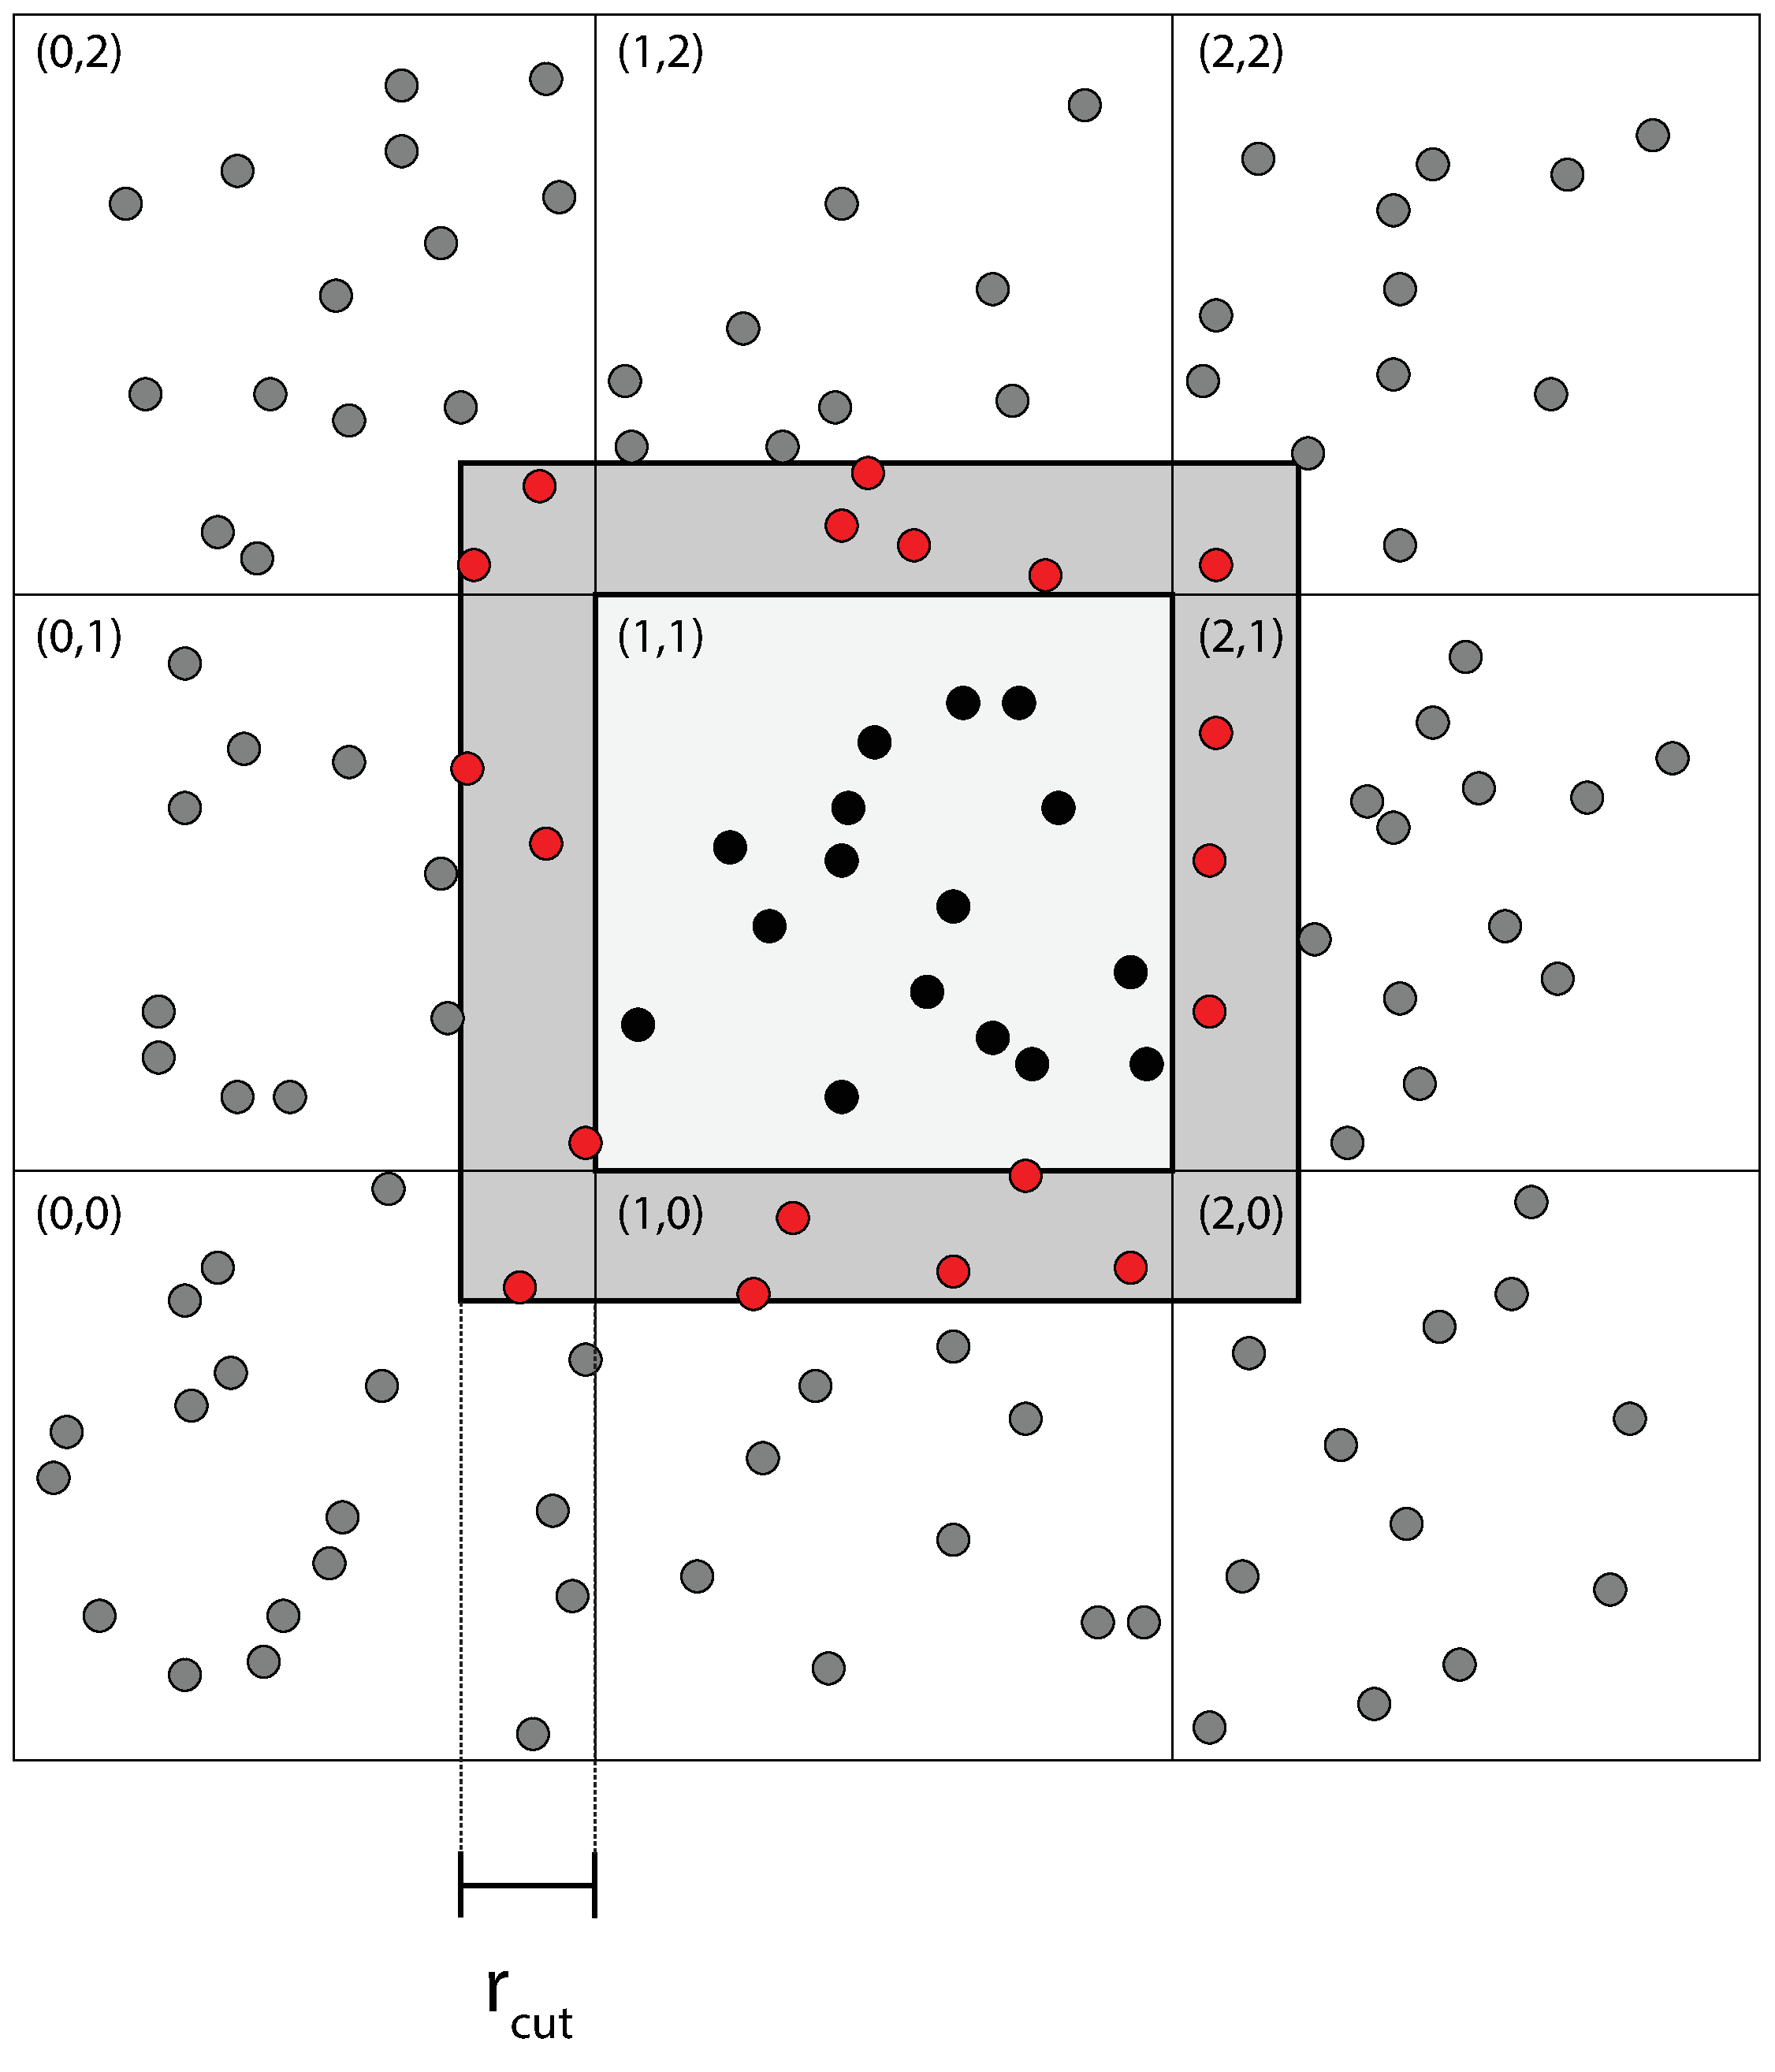
\includegraphics[width=0.8\textwidth, trim=0cm 0cm 0cm 0cm, clip]{MD/figures/parallelization_ghost_atoms.eps}
\end{center}
\caption{The middle processor with coordinates (1,1) in a two-dimensional system recieves a copy of all the atoms less than $r_\text{cut}$ from the boundary (ghost atoms, marked red) from the neighboring eight processors. The gray area is the region with the ghost atoms. The black dots are the atoms on node $(1,1)$, gray dots are atoms that do not contribute to the forces of the black atoms.}
\label{fig:md_ghost_atoms}
\end{figure}
Since we don't calculate forces between atoms displaced by more than the cut-off radius, we actually compute all the forces we want. This process is done for every processor, every timestep, so that all nodes have all the information they need to compute the forces (and potential energy).
\subsection{Cell lists}
We will now sort the atoms on a node into cells, similar to the collision cells in DSMC (see section \ref{sec:dsmc_implementation_timestep}). Each processor has atoms with coordinates in the range $[0, l_i)$, $l_i$ being the node length in the $i$th dimension, and ghost atoms with coordinates $(-r_\text{cut}, 0) \cup [l_i, l_i + r_\text{cut})$. We choose the cells to be about the same size as the cut-off radius, which gives the number of such cells $N_f$ (force cells) in the $i$th dimension
\begin{align}
	N_f = \ceil{l_i / r_\text{cut}} + 2,
\end{align}
where we have added two extra \textit{ghost cells} containing the ghost atoms, $\ceil{a}$ is the ceiling function of $a$, that is, the smallest integer number not larger than $a$. The reason we use the ceiling function is so the length of the node exactly matches the combined length of the cells (minus the two extra ghost cells). The size of the cells is then at least $r_\text{cut}$ so that the atoms within a cell will not feel the presence of atoms from any other cells than the 26 nearest neighbors. In figure \ref{fig:md_cells} we have illustrated the idea in a two-dimensional system. We see the total spatial domain of a processor with the copied ghost atoms (in the gray area), divided into cells of size $r_\text{cut}$. The yellow cell will compute forces between all of its atoms and the atoms in the green cells. This is done for every inner cell (the ghost atoms are computed on another processor).
\begin{figure}[h]
\begin{center}
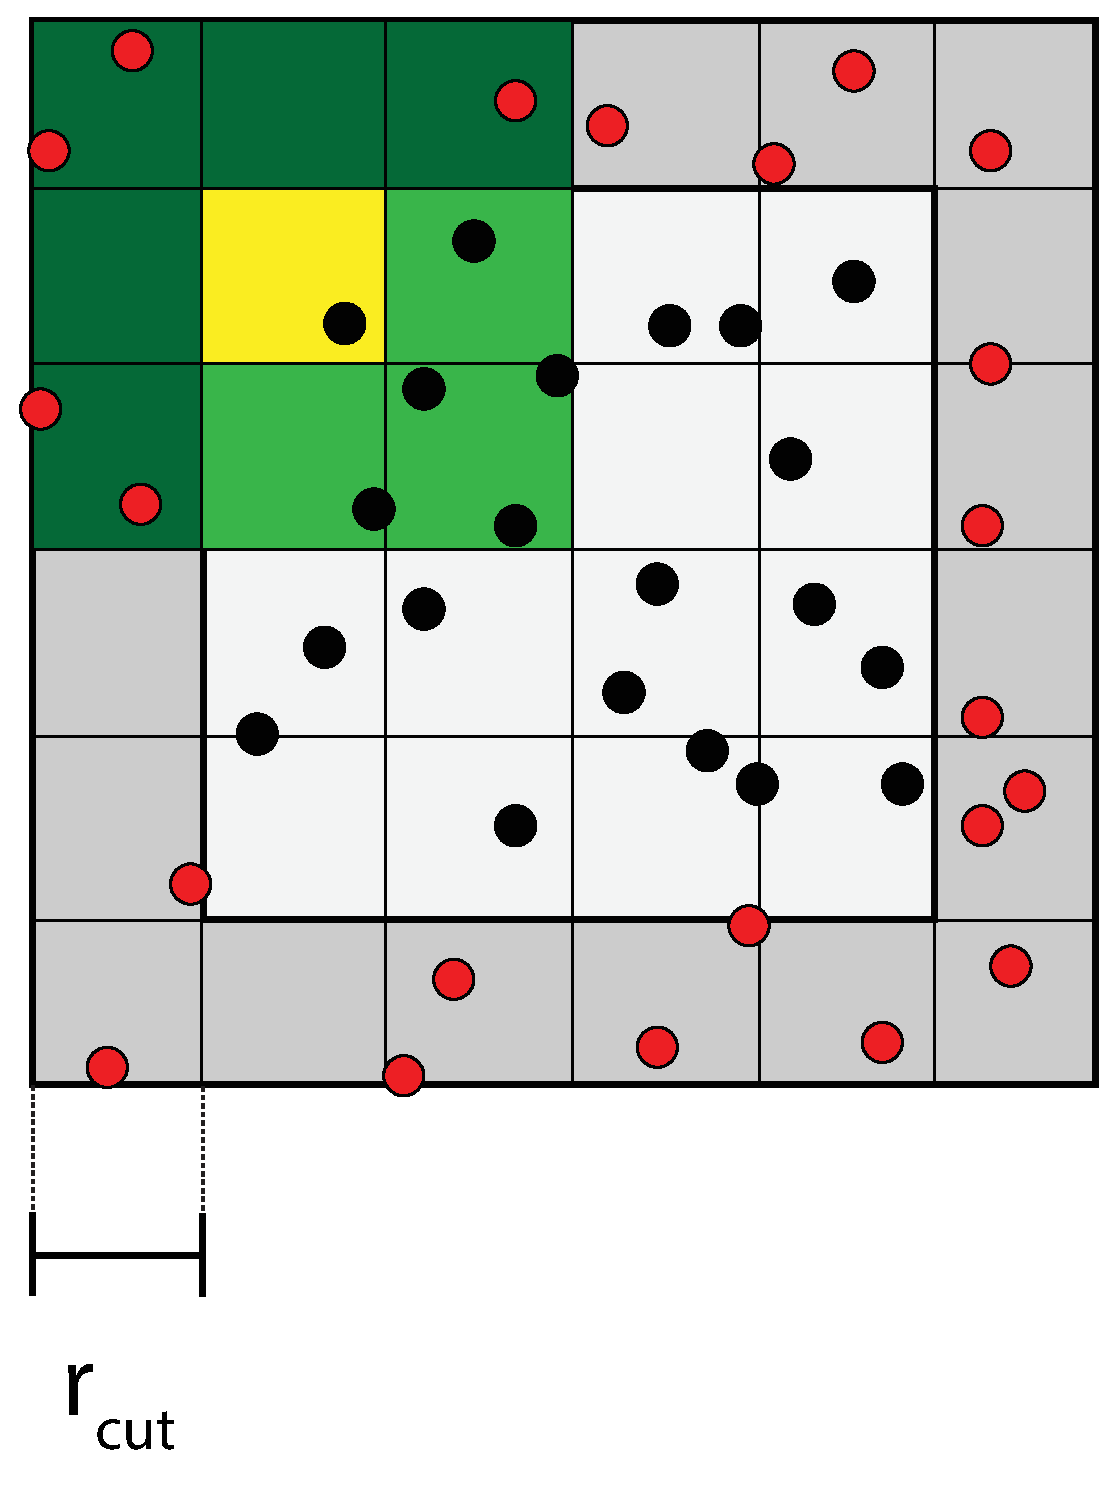
\includegraphics[width=0.8\textwidth, trim=0cm 0cm 0cm 0cm, clip]{MD/figures/cells.eps}
\end{center}
\caption{The spatial domain for a processor with the added ghost atoms in the gray area. The domain is divided into cells of size $r_\text{cut}$ so that the yellow cell only needs to compute forces between atoms in the cell and the neighboring 8 green cells. The processor will only process the cells (the ghost atoms are computed on another processor).}
\label{fig:md_cells}
\end{figure}
\subsection{Calculation of forces}
The atoms are now sorted into cells. We then loop over all cells, and for each cell, loop over the 26 neighboring cells. With each cell pair, loop over all pairs of atoms and calculate forces between them if their relative distance is smaller than $r_\text{cut}$. In the inner scope of the loop, we now have two atoms $i$ and $j$ with positions $\vec r_i$ and $\vec r_j$. Given their relative distance $\vec r_{ij} = (\Delta x, \Delta y, \Delta z)$, we are ready to compute the force between them. The Lennard-Jones force is given as (for $r_{ij} \leq r_\text{cut}$)
\begin{align}
	\vec F(\vec r_{ij}) = -24\epsilon\left[2\left(\frac{\sigma^{12}}{r_{ij}^{13}}\right) - \left(\frac{\sigma^6}{r_{ij}^7}\right)\right]\vec u_{ij},
\end{align}
and if we choose the so-called MD units ($\sigma = 1.0, \epsilon = 1.0$, see appendix \ref{app:physical_units}), the $x$-component of the force is given as
\begin{align}
	\label{eq:md_implementation_timestep_lj}
	F_x(r_{ij}) = -24\left[\left(\frac{2}{r_{ij}^{12}}\right) - \left(\frac{1}{r_{ij}^6}\right)\right]\frac{\Delta x}{r_{ij}^2},
\end{align}
where $\Delta x$ is the $x-$component of $\vec r_{ij}$. Notice that we have factored out $1/r_{ij}^2$. This is arithmetical convenient for the implementation, because, as we see in equation \eqref{eq:md_implementation_timestep_lj}, we need $r_{ij}^{-6}$ and $r_{ij}^{-12}$, which both are easily calculated from $r_{ij}^{-2}$ as powers.\\
First, we skip atoms displaced by a distance larger than $r_\text{cut}$ and compute the square of the relative distance
\begin{align}
	r_{ij}^2 = \left|\vec r_i - \vec r_j\right|^2.
\end{align}
Its inverse is gives us the higher powers
\begin{align}
	r_{ij}^{-2} &= \frac{1}{r_{ij}^2}\\
	r_{ij}^{-6} &= \left(r_{ij}^{-2}\right)^3\\
	r_{ij}^{-12} &= \left(r_{ij}^{-6}\right)^2.
\end{align}
In listing \ref{lst:md_lennard_jones} we have shown the code that calculates the Lennard-Jones force. We see that Newton's third law is implemented by skipping a pair of atoms if \classname{atom\_index\_0}<\classname{atom\_index\_1}, avoiding calculating that pair twice. 
\begin{lstlisting}[caption=Implementation of the Lennard-Jones force. The code loops over all cells and their neighbors computing the forces between all the atoms in neighboring cells., label=lst:md_lennard_jones]
void calculate_lennard_jones() {
    // Loop through all local cells (not including ghosts)
    for (int cell_index_x=1; cell_index_x<=num_cells.x; cell_index_x++) {
    for (int cell_index_y=1; cell_index_y<=num_cells.y; cell_index_y++) {
    for (int cell_index_z=1; cell_index_z<=num_cells.z; cell_index_z++) {
    // Index of this cell
    cell_index = cell_index_from_ijk(cell_index_x, cell_index_y, cell_index_z);

    // Loop through all neighbors (including ghosts) of this cell.
    for (int i=cell_index_x-1; i<=cell_index_x+1; i++) {
    for (int j=cell_index_y-1; j<=cell_index_y+1; j++) {
    for (int k=cell_index_z-1; k<=cell_index_z+1; k++) {
    // Index of neighbor cell
    cell_index_2 = cell_index_from_ijk(i,j,k);
    // Head is pointing to the first atom index in a cell
    int atom_index_0 = head_atoms[cell_index]; 

    while (atom_index_0 != EMPTY) { // The last atom in a cell points at the EMPTY value
    int atom_index_1 = head_atoms[cell_index_2]; // Index of atom j
    while (atom_index_1 != EMPTY) {
        if(atom_index_0 < atom_index_1) { // Newton's 3rd law
            double dx = positions.at(atom_index_0).x-positions.at(atom_index_1).x;
            double dy = positions.at(atom_index_0).y-positions.at(atom_index_1).y;
            double dz = positions.at(atom_index_0).z-positions.at(atom_index_1).z;
            
            double dr2 = dx*dx + dy*dy + dz*dz;

            if (dr2<r_cut_squared) {
                double dr2_inverse = 1.0/dr2;
                double dr6_inverse = dr2_inverse*dr2_inverse*dr2_inverse;
                double dr12_inverse = dr6_inverse*dr6_inverse;
                double force = 24*(2*dr12_inverse-dr6_inverse)*dr2_inverse;

                accelerations.at(atom_index_0).x += force*mass_inverse*dx;
                accelerations.at(atom_index_0).y += force*mass_inverse*dy;
                accelerations.at(atom_index_0).z += force*mass_inverse*dz;

                accelerations.at(atom_index_1).x -= force*mass_inverse*dx;
                accelerations.at(atom_index_1).y -= force*mass_inverse*dy;
                accelerations.at(atom_index_1).z -= force*mass_inverse*dz;
            }
        }
        atom_index_1 = linked_list_of_atoms[atom_index_1]; // Next
    }
    atom_index_0 = linked_list_of_atoms[atom_index_0];
    }}}}}}}
}
\end{lstlisting}